\chapter{Infraestructura Software} 

Una vez presentados los objetivos que tenemos marcados hay que echar una mirada a las tecnologías software y hardware que hemos utilizado como base en el proyecto. La más importante y sobre la que está centrado el proyecto es WebRTC. Además hemos empleado, como apoyo para cubrir las partes a las que WebRTC no llega, ICEJS junto con la plataforma robótica JdeRobot. Estas tecnologías junto con el simulador robótico Gazebo nos han permitido probar, depurar y mejorar el código antes de realizar los experimentos sobre el drone real ArDrone, el cuál presento a continuación.\\


\section{ArDrone de Parrot}

El Parrot\footnote{\url{http://www.parrot.com/es/productos/ardrone-2/}} ARDrone es un drone que comercializa la marca Parrot el cuál puede ser teleoperado con una aplicación desde dispositivos móviles. El drone crea una red WiFi, a la cuál conectas tu teléfono o tablet iOS ó Android y desde la aplicación, suministrada también por la marca Parrot,  se tiene una comunicación directa con el drone.\\

A parte de esto Parrot tiene una SDK para desarrolladores la cuál es libre y está muy bien documentada para que quien quiera pueda desarrollar sus aplicaciones. Esta SDK es sobre la que JdeRobot ofrece, junto con el middleware ICE (\emph{Internet Communication Engine}), una pasarela que nos da conectividad entre el drone real y la aplicación/componente que estemos desarrollando o usando.\\

\begin{figure}[h!]
\centering
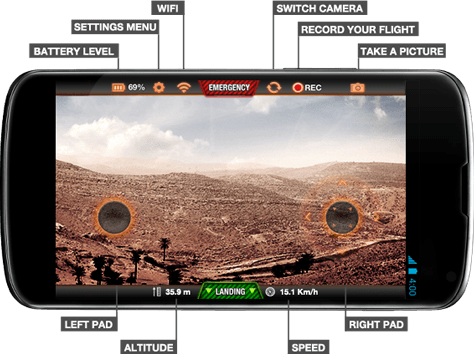
\includegraphics[width=0.6\textwidth]{ardrone_movil}
\end{figure}

\begin{figure}[h!]
\centering
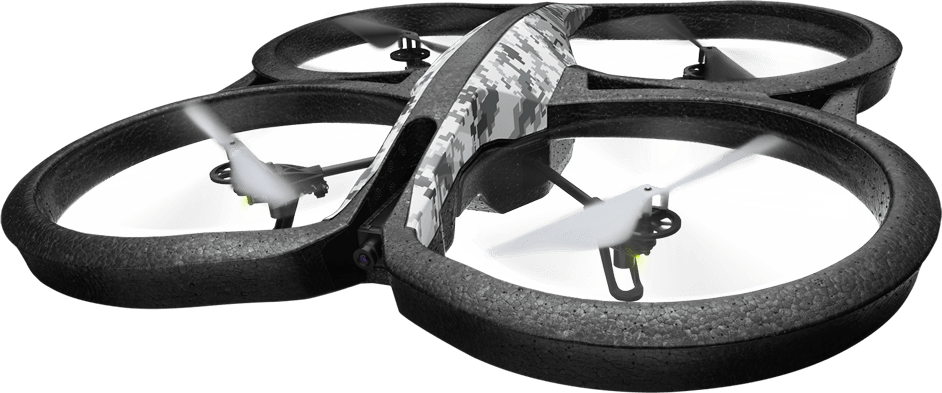
\includegraphics[width=0.6\textwidth]{ardrone}
\caption{ArDrone de Parrot}
\label{fig:ardrone}
\end{figure}

Para este proyecto hemos usado la versión ArDrone 2.0, el cuál cuenta como principales características de una cámara HD a 720p y 30fps y una altitud máxima de vuelo de 100 metros de altura. Tiene una autonomía de vuelo de aproximadamente 11-12 minutos, y su carga máxima de pago ronda los 400 gramos de peso. En su interior tiene un microprocesador AR M Cortex A8 de 32 bits a 1GHz con DSP de vídeo a 800MHz el cuál corre Linux en su interior. En este proyecto usaremos el ArDrone 2.0 para conectar un navegador web externo con el microprocesador que corre a bordo del drone y teleoperarlo a distancia.\\

Para simular este drone de una manera realista y realizar las pruebas de manera virtual, nos vamos a apoyar en el simulador robótico Gazebo.\\


\section{Simulador robótico Gazebo}

Gazebo\footnote{\url{http://gazebosim.org}} es un simulador 3D de robótica desarrollado por la \textit{Open Source Robotics Foundation (OSRF)}. Es multiplataforma y entre otras cosas nos permite diseñar y crear nuestro propio robot y escenarios realistas, con obstáculos y objetos, para probar nuestros algoritmos de una forma parecida a las condiciones que vamos a encontrar en el mundo real, pero sin poner en peligro ni nuestros robots ni a ninguna persona cercana en caso de que se comporte de una forma inesperada. Para conseguir este realismo y potencia Gazebo cuenta con un motor físico para la mecánica, iluminación, gravedad, inercia... Uno de los puntos más favorables de este simulador es que es libre y tiene una comunidad muy numerosa y participativa.\\

JdeRobot tiene desarrollado el plugin para Gazebo que contiene el modelo, el mundo y los interfaces necesarios para simular el ArDrone de Parrot, de tal manera que podremos probar el código para ir puliendo y conseguir que sea lo suficientemente estable antes de probarlo en el drone real.\\

Se ha usado la versión 5.1 del simulador, la cuál es última version estable a la fecha de comienzo del TFG y 100\% compatible con el plugin de JdeRobot mencionado, el cuál se explica a continuación en mayor profundidad.\\

\begin{figure}[h!]
\centering
\includegraphics[width=0.8\textwidth]{gazebo}
\caption{Simulador Gazebo}
\label{fig:gazebo}
\end{figure}

Este simulador junto con los plugins, mundos y mapas creados por JdeRobot es una poderosa herramienta que nos será muy útil para nuestro proyecto.\\

\section{JdeRobot}

JdeRobot\footnote{\url{http://jderobot.org}}\cite{jderobot} es un proyecto desarrollado por el laboratorio de robotica de la Universidad Rey Juan Carlos. Es un entorno para el desarrollo de aplicaciones relacionadas con la robotica, la visión artificial, automatización del hogar y escenarios con sensores y actuadores, y software inteligente. Está escrito mayormente en C++ y basado en un entorno de componentes distribuidos. Los componentes, que pueden correr de manera simultánea de manera asíncrona están conectados a través del \emph{middleware} ICE, el cuál veremos a continuación. Los componentes pueden ser escritos en C++, Java, Python... y todos ellos interoperan a través de interfaces ICE.\\

JdeRobot simplifica el acceso a unidades hardware como cámaras. Obtener datos de un sensor es tan sencillo como llamar a una función local, y mandar comandos a un motor o actuar se hace también simplemente llamando a una función local. Estos sensores, actuadores o unidades hardware pueden ser simuladas o reales y estar en local o en una red como internet.\\

Incluye numerosas librerías y herramientas que podemos usar para desarrollar nuestra propia aplicación o para controlar nuestro propio robot. JdeRobot es software libre, bajo licencia GPL y LGPL. También utiliza software de terceros como el simulador Gazebo, ROS, GTK, OpenCV...\\

La versión utilizada en el proyecto ha sido la 5.3.1, última versión estable en la fecha del comienzo del mismo. Dentro de las herramientas utilizadas en el proyecto hemos hecho uso básicamente de dos:

\begin{itemize}
\item \emph{Plugin de Gazebo}: Desarrollado para añadir el ArDrone a Gazebo con las mismas funcionalidades que el drone real. Este plugin nos permite abstraernos de las conexiones a más bajo nivel, como la lectura de sensores o en envío de comandos a los motores, simplificando el acceso a los mismos y obteniendo los datos con una simple llamada a función.

\item \emph{ArDroneServer}: Este componente es el encargado de comunicarse directamente con el ArDrone real, ejecutar las funciones y comandos de bajo nivel para obtener los datos y valores de los sensores, y ejecutar las funciones necesarias sobre los motores y actuadores según las órdenes de movimiento dadas. De cara al usuario ofrece seis interfaces ICE, a las que puedes conectar tu aplicación. En la figura \ref{fig:ardroneserver} puedes ver la estructura general del componente.
\end{itemize}

\begin{figure}[h!]
\centering
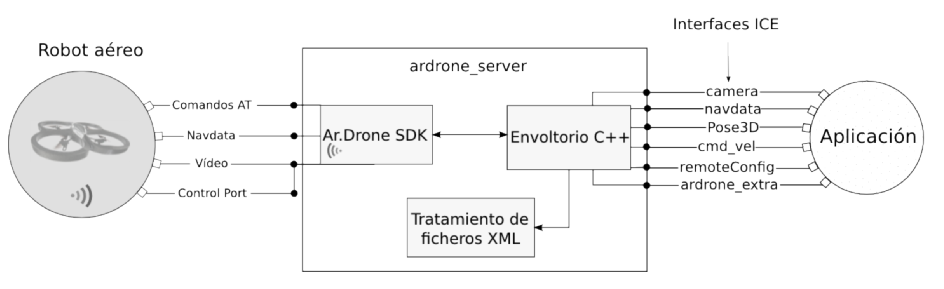
\includegraphics[width=1\textwidth]{ardroneserver}
\caption{Estructura de ArDrone\_Server}
\label{fig:ardroneserver}
\end{figure}

\section{ICE}

ICE\footnote{https://zeroc.com} o \emph{Internet Communication Engine} es un entorno RPC orientado a objetos desarrollado por la empresa Zeroc con soporte para lenguajes como C++, C\#, Java, JavaScript, y Python entre otros, y SO's como Linux, Mac OS X y Windows, que nos permite crear conexiones e interacciones de red entre máquinas con servidores corriendo en diferentes lenguajes y/o SO's. Estas conexiones pueden ser síncronas o asíncronas, usando variedad de protocolos de red como TCP, UDP ó SSL/TTS\\

ICEJS, o ICE for JavaScript es un \textit{plugin} que se le puede añadir a ICE el cual añade la funcionalidad de conexiones mediante \textit{websockets} lo que nos permite conectar navegadores a través de JavaScript a los protocolos más comunes de ICE. \\

En versiones más actuales ICEJS viene incorporado en la suite principal de ICE, pero nosotros hemos usado la versión 3.5 que es la que soporta la suite de JdeRobot con la que trabajamos, por lo que debemos instalar el plugin una vez instalado ICE.\\

\begin{figure}[h!]
\centering
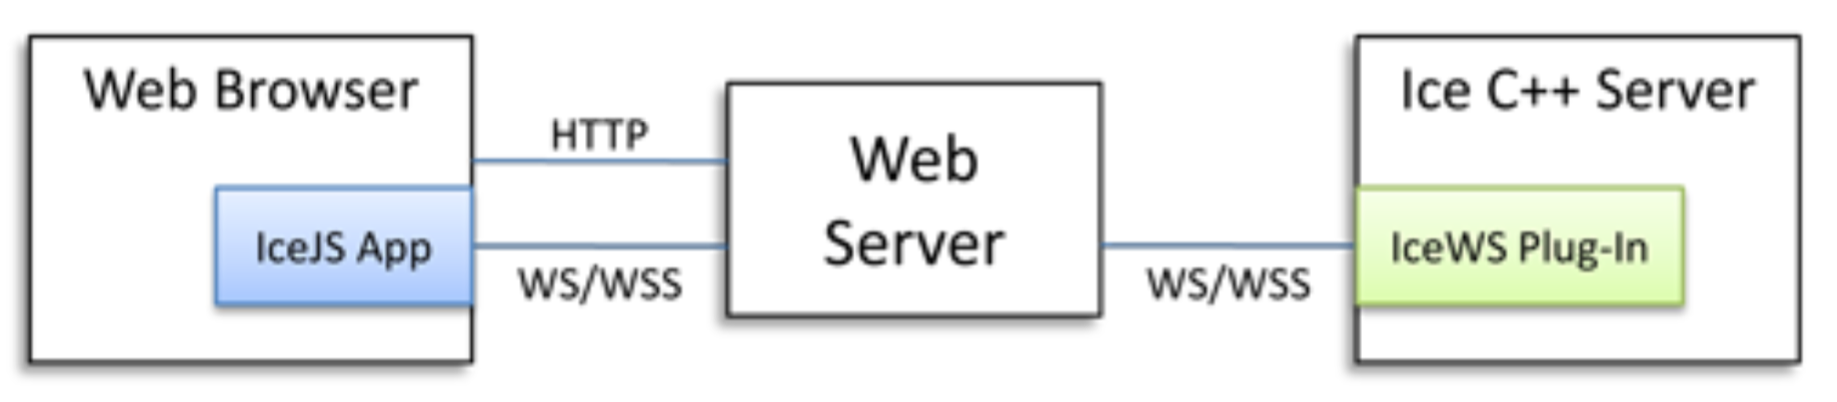
\includegraphics[width=0.8\textwidth]{esquema_icejs}
\caption{Esquema de ICE JS}
\label{fig:esquema_icejs}
\end{figure}

\section{WebRTC}

Web Real-Time Communication\footnote{\url{https://webrtc.org}}\cite{Pagina WebRTC} (WebRTC) es un proyecto de software libre y gratuito que nos permite tener en el navegador tecnología en tiempo real ('Real-Time Communication' ó RTC) sin plugins, a través de varias APIs de JavaScript. Facilita las llamadas de voz, videollamadas, chat y compartición de archivos y datos. WebRTC es una tecnología entre pares, por lo que permite desarrollar estas aplicaciones para que funcionen directamente desde un navegador a otro \emph{sin pasar por servidor intermedio} para el trasiego de datos.\\

En todo el documento nos referimos a una llamada WebRTC entre dos navegadores, lo cual es su principal propósito, pero también está diseñado para que pueda ser integrado con otros sistemas de comunicación como voz sobre IP (VOIP), clientes SIP, e incluso sobre la red telefónica pública conmutada (PSTN).\\

Enviar audio y/o vídeo con calidad e intercambiar cualquier tipo de datos requiere de muchas funcionalidades complejas en el navegador. Para no preocuparnos de estas dificultades las APIs de WebRTC proporcionan todo el conjunto completo de funciones para manejar y crear nuestras aplicaciones, como el control y administración de la conexión, codificación/decodificación del audio/vídeo, negociación entre navegadores, control de la conexión, atravesar cortafuegos y NATs.\\

Con unas docenas de líneas de JavaScript podemos tener una videoconferencia entre pares con intercambio de archivos o datos en tiempo real. Ese es el potencial que WebRTC tiene. Pero aún así hay una serie de escollos como la señalización, descubrimiento de pares, negociación de la conexión o seguridad que debemos controlar para conseguir una llamada exitosa.\\

Que WebRTC no necesita un servidor no es del todo cierto, ya que sí que necesita de lo que llamamos Servidor de Señalización. Éste es el encargado de establecer el primer contacto entre los pares, facilitando el intercambio de paquetes de la negociación WebRTC.\\

\noindent WebRTC está compuesto de 3 API's:

\begin{itemize}
\item \emph{getUserMedia}: para la adquisición del flujo local de audio y vídeo.
\item \emph{RTCPeerConnection}: para la comunicación de audio y vídeo.
\item \emph{RTCDataChannel}: para la comunicación de cualquier otro tipo de datos.
\end{itemize}

En este momento WebRTC es accesible para todos los usuarios a través de navegadores como Chrome o Firefox. Sin embargo, WebRTC está aún en construcción, tanto la forma de implementar las API's que tiene cada navegador como la propia norma, con sus protocolos de funcionamiento. Como resultado todo lo que exponga sobre estas API's se refiere a la situación actual y puede cambiar en el futuro.\\

En las siguientes secciones vamos a desgranar y explicar con detalle cómo funciona el intercambio de paquetes de señalización así como cada una de las API's que componen WebRTC.\\

\section{WebRTC: Señalización} 
\label{sec:senalizacion}

Señalización es el proceso de intercambio de datos y metadatos necesarios para coordinar una llamada entre navegadores con WebRTC. Para realizar esta labor WebRTC necesita de la ayuda de un servidor externo ya que la norma deja el campo de la señalización a la capa de la aplicación.\\

Los objetivos básicos de la señalización son dos, el intercambios de los datos necesarios para establecer un flujo audiovisual y el intercambio de direcciones de red para que los pares sean alcanzables. Entre las labores para satisfacer estos objetivos se encuentran la detección de los pares, el intercambio de paquetes de control de la sesión como los candidatos \emph{ICE (Internet Communication Engine)} y los \emph{SDP (Session Description Protocol)}, las prestaciones que puede darnos cada par así como cualquier otro dato o paquete necesario para realizar este 'apretón de manos' inicial.\\

WebRTC no especifica qué tipo de servidor hemos de usar para estas funciones. Esto es debido a que diferentes aplicaciones pueden preferir distintos servidores básicos o personalizados según sus necesidades. La única restricción es el uso de la arquitectura JSEP, la cuál especifica cómo debe ser la secuencia de señalización para tener una llamada exitosa.\\


El servidor debe usar la arquitectura \emph{JSEP (JavaScript Session Establishment Protocol)}. Esta arquitectura elimina al navegador de casi todo el flujo de señalización, el cual se maneja desde JavaScript haciendo uso de dos interfaces: transfiriendo los SDP local/remoto e interactuando con la máquina de estados ICE. Esta arquitectura nos evita, entre otras cosas, que el navegador tenga que guardar estados de sesión, de tal manera que se pueden guardar en el servidor y evitar problemas si la página se recarga, por ejemplo. \\

JSEP no establece un modelo particular de señalización más allá de usar uno capaz de realizar el intercambio de los SDP y ICE según la norma RFC3264 de \emph{oferta/respuesta}, [(figura \ref{fig:oferta-respuesta})] de tal manera que ambas partes de la llamada sepan cómo actuar en cada momento. JSEP nos da los mecanismos necesarios para crear estas ofertas, así como aplicarlas a las sesión.\\

\begin{figure}[h!]
\centering
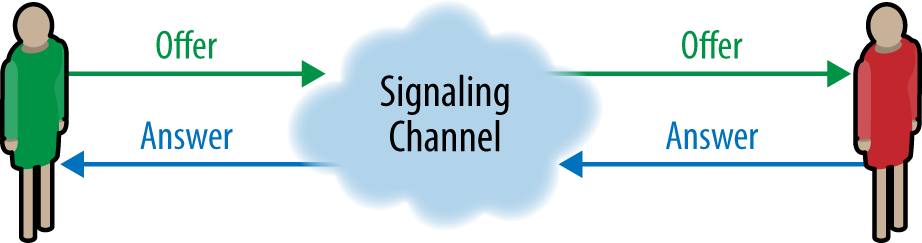
\includegraphics[width=0.9\textwidth]{offer-answer}
\caption{Oferta / Respuesta a través del servidor de señalización}
\label{fig:oferta-respuesta}
\end{figure}


El orden en que se llaman a estos mecanismos o funciones de la API es importante, por lo que la aplicación deberá saber el orden en el que tiene que llamar a cada una, convertir las ofertas en mensajes que entienda el protocolo de señalización elegido y hacer la conversión inversa con los mensajes que se reciben para obtener ofertas que entiendan las API's.\\


\subsection{Estableciendo el Flujo Audiovisual: Descriptores de Sesión}

Para establecer un intercambio de flujo audiovisual, el \textit{agente de usuario (user agent)} del navegador necesita parámetros específicos para indicar al par remoto qué es lo que va a transmitir, de la misma manera que necesita conocer los parámetros del flujo audiovisual que va a recibir para saber cómo decodificarlo y manejarlo. Estos datos se determinan en la descripción de sesión (SDP), los cuales se intercambian en ofertas/respuestas usando las API's JSEP como ya hemos visto anteriormente.\\

El manejo de las descripciones de sesión es simple y sencillo. Siempre que el intercambio de una oferta/respuesta es necesario, el par que establece la llamada ó \textit{llamante (callee)} crea la oferta llamando a la función \emph{createOffer()} de la API. Esta oferta puede ser modificada por la aplicación si así fuese necesario. Se establece como configuración local en ese par con \emph{setLocalDescription()} y se envía al par remoto a través del servidor de señalización utilizado. Al recibir esta oferta el par \textit{llamado (called)} lo utiliza como configuración del otro par con \emph{setRemoteDescription()} y utiliza \emph{createAnswer()} para crear una respuesta apropiada, la cual establece como configuración local (\emph{setLocalDescription()}) y envía la respuesta de vuelta a través del servidor de señalización. El par llamado al recibir la respuesta llama también a \emph{setRemoteDescription()}, y de esta manera ambos lados tienen la información del descriptor de sesión propio y el del par remoto.\\ 



Si el SDP pertenece a la parte local o remota tiene su importancia. Una vez realizado el intercambio, cada parte mirará la lista de codecs soportados por él mismo y por la otra parte, y el cruce de los resultados determinará qué codecs debe usar para enviar y cuál para digerir lo recibido. Los parámetros exactos de la transmisión sólo se pueden saber una vez la oferta y la respuesta han sido intercambiados. Sin embargo, hay ocasiones en las que el llamante o el que hace la oferta puede recibir flujo audiovisual después de enviar la oferta pero antes de recibir la respuesta proveniente del otro par. Para procesar este flujo audiovisual de manera adecuada, el manejador del llamante debe conocer los detalles de la oferta antes de que la respuesta llegue.\\

Por lo tanto, para manejar los descriptores de sesión de manera correcta, los agentes de usuario necesitan:

\begin{itemize}
\item Conocer si el descriptor de sesión pertenece a la parte local o remota.
\item Conocer si el descriptor de sesión es una oferta o una respuesta.
\item Permitir a la oferta ser especificada independientemente de la respuesta.
\end{itemize}

Para satisfacer estas premisas JSEP aborda esto añadiendo los métodos \emph{setLocalDescription()} y \emph{setRemoteDescription()} y teniendo un campo en los descriptores de sesión indicando el tipo de sesión que se suministra. En la figura \ref{fig:sdp-oferta-respuesta} podemos ver el esquema de intercambio de paquetes SDP y el ajuste de los mismos en cada par según corresponde.\\

\begin{figure}[h!]
\centering
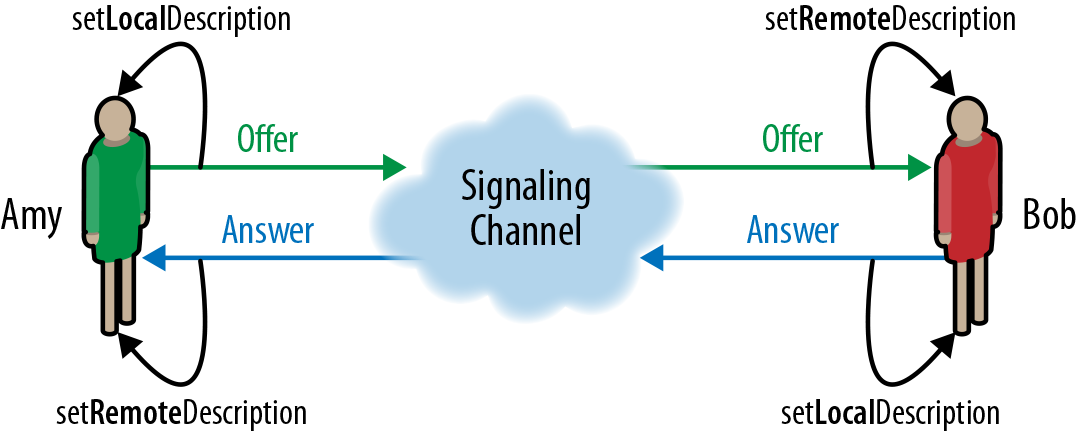
\includegraphics[width=0.9\textwidth]{SDP_offer-answer}
\caption{Intercambio y establecimiento de los SDP en cada par.}
\label{fig:sdp-oferta-respuesta}
\end{figure}

JSEP también permite el uso de respuestas provisionales. Estas respuestas permiten al par remoto o llamado comunicar e informar de los parámetros iniciales de la sesión al llamante, de tal manera que la sesión puede comenzar mientras se espera una respuesta final posteriormente. Este concepto es importante en el modelo oferta/respuesta, ya que al recibir una de estas respuestas el llamante puede liberar y usar más recursos como extra \textit{candidatos ICE, candidatos TURN} o vídeo decodecs. Estas respuestas provisionales no provocan ningún tipo de des-asignación o problema, por lo que pueden ser recibidas a lo largo de la llamada para estabilizar o mejorar la misma según varíen las condiciones del ancho de banda de uno de los pares, por ejemplo.\\

\subsubsection{Formato de los Descriptores de Sesión}

En la especificación WebRTC, los descriptores de sesión o \emph{session descriptions} están formados por mensajes \textit{SDP (Session Description Protocol)}. Este formato no es el óptimo para manipular con JavaScript, pero es el más popular y aceptado en el campo de las comunicaciones audiovisuales en tiempo real. Este formato es el que usa JSEP para formar e intercambiar los descriptores de sesión.\\

Para facilitar el procesado en JavaScript y una futura flexibilidad, los SDP los genera la API como un objeto o \textit{blob}. Si en un futuro WebRTC soporta algún formato nuevo para los descriptores de sesión, estos serán fácilmente añadidos y habilitados para poder usarlos en nuestras aplicación en vez de SDP.\\

La forma que tiene un paquete SDP es la siguiente:

\begin{lstlisting}[caption=Ejemplo paquete SDP]
v=0
o=- 7729291447651054566 1 IN IP4 0.0.0.0
s=-
t=0 0
a=group:BUNDLE a1 d1
a=ice-options:trickle
m=audio 9 UDP/TLS/RTP/SAVPF 96 0 8 97 98
c=IN IP4 0.0.0.0
a=rtcp:9 IN IP4 0.0.0.0
a=mid:a1
a=msid:QI39StLS8W7ZbQl1sJsWUXkr3Zf12fJUvzQ1
       QI39StLS8W7ZbQl1sJsWUXkr3Zf12fJUvzQ1a0
a=sendrecv
a=rtpmap:96 opus/48000/2
a=rtpmap:0 PCMU/8000
a=rtpmap:8 PCMA/8000
a=rtpmap:97 telephone-event/8000
a=rtpmap:98 telephone-event/48000
a=maxptime:120
a=ice-ufrag:7sFvz2gdLkEwjZEr
a=ice-pwd:dOTZKZNVlO9RSGsEGM63JXT2
a=fingerprint:sha-256 6B:8B:F0:65:5F:78:E2:51:3B:AC:6F:F3:3F:46:1B:35
                     :DC:B8:5F:64:1A:24:C2:43:F0:A1:58:D0:A1:2C:19:08
a=setup:active
a=rtcp-mux
a=rtcp-rsize
a=extmap:1 urn:ietf:params:rtp-hdrext:ssrc-audio-level
a=extmap:2 urn:ietf:params:rtp-hdrext:sdes:mid
a=imageattr:97 send [x=[128:16:1280],y=[72:9:720]] recv [x=[128:16:1280],y=[72:9:720]]
a=ssrc:4429951804 cname:Q/NWs1ao1HmN4Xa5

m=application 9 UDP/DTLS/SCTP webrtc-datachannel
c=IN IP4 0.0.0.0
a=mid:d1
a=fmtp:webrtc-datachannel max-message-size=65536
a=sctp-port 5000
a=fingerprint:sha-256 6B:8B:F0:65:5F:78:E2:51:3B:AC:6F:F3:3F:46:1B:35
                     :DC:B8:5F:64:1A:24:C2:43:F0:A1:58:D0:A1:2C:19:08
a=setup:active
\end{lstlisting}

El cometido principal del intercambio de SDP es la negociación de vídeo. Es un proceso a través del que cada par puede indicar al otro qué resoluciones y \textit{frames rate} de vídeo es capaz de recibir. Esto lo hace a través del atributo \textit{'a=imageattr'} en el SDP. Cada par puede tener límites como la capacidad de proceso que el decoder tiene, o simplemente restricciones de la aplicación.\\


\subsection{Intercambio de los Datos de Red: Interactive Connectivity Establishment (ICE)}

Al igual que los pares tienen que intercambiar información sobre el media, también necesitan hacerlo sobre la información de \textit{red} para que los pares sean visibles entre ellos y puedan alcanzarse. ICE es una técnica usada en aplicaciones de voz, vídeo, \emph{peer-2-peer}, entre otros que nos permite solucionar problemas de alcance de red entre dos ordenadores. Estos problemas son debidos a que los ordenadores suelen estar dentro de una red privada y/o cortafuegos. Esta técnica nos permite descubrir suficiente información sobre la topología de los otros pares para encontrar una o varias rutas potenciales entre ellos, preferiblemente directas.\\

Esta información ha de obtenerse de manera local en cada par con el \textit{Agente ICE} asociado a cada objeto RTCPeerConnection. El Agente ICE es responsable de: 

\begin{itemize}
\item Reunir tuplas candidatas de IP + Puerto.
\item Realizar pruebas de conectividad entre los pares.
\item Enviar \textit{keepalives}.
\end{itemize}

Una vez se ha finalizado y configurado el proceso de descripción de sesión, el Agente ICE local comienza automáticamente el proceso de descubrir todos los posibles candidatos en el par local. A cada candidato posible se le llama \textit{Candidato ICE}:

\begin{enumerate}
\item El Agente ICE pide al sistema operativo las direcciones IP locales.
\item Consulta a un servidor \emph{STUN (Session Traversal Utilities for NAT}) externo la tupla de dirección IP pública y puerto del par.
\item Consulta a un servidor \emph{TURN (Traversal Using Relays around NAT)} como último recurso para hacer de intermediario trasegador de los datos multimedia. 
\end{enumerate}

Como podemos ver, ICE necesita de servidores externos para obtener la tupla de dirección IP y puerto públicos necesarios para el otro par si está fuera de la misma red local. STUN  es un protocolo estandarizado para descubrir direcciones IP públicas de equipos que están detrás de un NAT. TURN es un servidor para transmitir mensajes entre dos clientes. Este servidor sólo se usará si falla la conexión directa entre pares después de probar con las direcciones IP locales y las públicas obtenidas en el servidor STUN. No es obligatorio configurar estos servidores. Si la conexión entre los pares es en la misma red no necesitamos configurar servidores STUN/TURN ya que con las direcciones locales es suficiente.\\

\begin{figure}[h!]
\centering
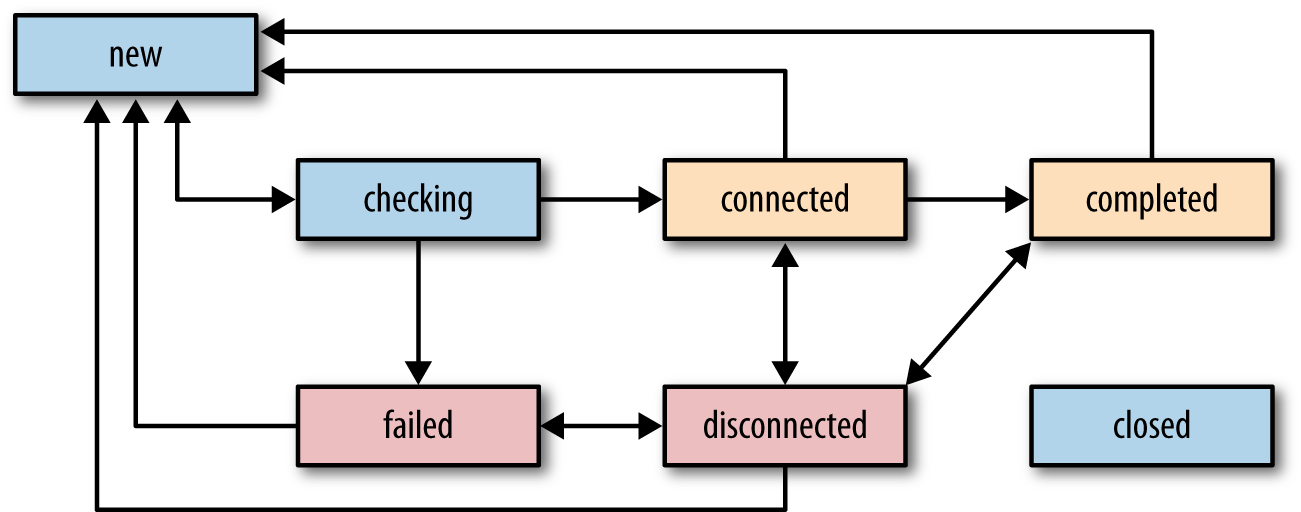
\includegraphics[width=0.9\textwidth]{estados-ICE}
\caption{Maquina de estados y transiciones ICE.}
\label{fig:estados-ice}
\end{figure}

 
Cuando un Candidato ICE es descubierto, se envía al par remoto y una vez allí, se añade en RTCPeerConnection la información de sesión que contiene ese paquete con \textit{setRemoteDescription()}, de tal manera que el Agente ICE puede empezar a hacer pruebas de conectividad para ver si puede alcanzar al otro par.\\

Una vez los dos Agentes ICE tienen una lista completa de los Candidatos ICE de ambos pares, cada agente comprueba emparejando ambas listas cuáles funcionan. Para ello tienen una planificación de prioridades: primero direcciones IP locales, luego IP públicas y finalmente si ambas fallan servidor TURN. Cada comprobación es una petición/respuesta STUN que el cliente realiza con un particular candidato enviando una petición STUN desde el candidato local al candidato remoto.\\

Si uno de los pares de candidatos funciona, entonces tenemos una ruta de conexión entre ambos pares. Si todos los candidatos fallan ambas conexiones RTCPeerConnection se marca como fallida o la conexión se hace a través de un servidor TURN.\\

Cuando una conexión se ha establecido correctamente cada Agente ICE continua haciendo peticiones STUN periódicas al otro par, lo cual sirve también como \textit{keepalives}.\\

\subsubsection{Goteo de Candidatos ICE \emph{(ICE Candidate Trickling)}}

Recopilar IP's locales es rápido, pero conseguir las IP's públicas con sus puertos a través de servidores STUN requiere de un intercambio de paquetes entre el par y el servidor STUN y por consiguiente más tiempo.\\

\emph{ICE Candidate Tricking} es una extensión del protocolo ICE por la cuál el llamante puede incrementar el número de candidatos para el llamado después de la primera oferta. Este proceso permite al llamado comenzar a establecer las conexiones ICE sin tener que esperar a que el llamante recopile todos los posibles candidatos. Con esta técnica conseguimos un establecimiento del flujo audiovisual más rápido.\\

Esta técnica es opcional aunque es la recomendada. Las aplicaciones que lo soportan pueden enviar directamente la oferta SDP inicial sin candidatos ICE inmediatamente, y enviar candidatos individuales cuando los vayan descubriendo; las aplicaciones que no lo soportan simplemente esperan la indicación de que la recopilación de candidatos está completa, crean la oferta con todos los candidatos y enviarla.\\

\begin{enumerate}
\item Intercambio ofertas SDP sin Candidatos ICE.
\item Cuando se descubre un candidato se envía directamente a través del servidor de señalización.
\item La comprobación de los Candidatos ICE se realiza en el momento de recibir uno.
\end{enumerate}

\subsubsection{Formato de un Candidato ICE}

\begin{lstlisting}[caption=Ejemplo paquete SDP]
candidate:1 1 UDP 1694498815 192.0.2.33 10000 typ host
\end{lstlisting}

\noindent \textbf{Fundación (1):} Identificador para cada candidato del mismo tipo, misma interfaz y servidor STUN.\\
\textbf{ID (1):} Identificador. 1 para RTP, 2 para RTCP.\\
\textbf{Protocolo (UDP):} Protocolo de transporte del candidato.\\
\textbf{Prioridad (1694498815): }Prioridad del componente dado.\\
\textbf{Dirección IP y puerto (192.0.2.33 10000): }Dirección IP y puerto del candidato.\\
\textbf{Tipo (typ):} Tipo del componente.\\
\textbf{Dirección relacionada (host):} Información opcional que contiene dirección IP y puerto privado.\\


\section{WebRTC: API getUserMedia} 

getUserMedia es la API encargada de suministrar el flujo de audio y/o vídeo. Pide permiso al usuario para acceder y utilizar los dispositivos hardware como la cámara y el micrófono. Por el momento sólo está disponible para captar el hardware de audio y vídeo anteriormente mencionado, pero se pretende mejorar y ampliar la API para que en un futuro se pueda hacer \emph{streaming} de casi cualquier fuente de datos, como un disco duro o sensores conectados al ordenador.\\

Para tener una rica videoconferencia no es suficiente con obtener los flujos en crudo \textit{ó formato raw} de la cámara o el micrófono. Cada flujo debe ser procesado para aumentar la calidad, sincronizarlos y ajustar el caudal \textit{(bitrate)} de salida según las fluctuaciones del ancho de banda y la latencia entre pares. A la hora de recibir el flujo nos encontramos en la misma situación pero a la inversa. WebRTC nos da unos motores de procesado de audio y vídeo (figura \ref{fig:audio-video_engines}) que harán todas estas cosas por nosotros.\\

\begin{figure}[h!]
\centering
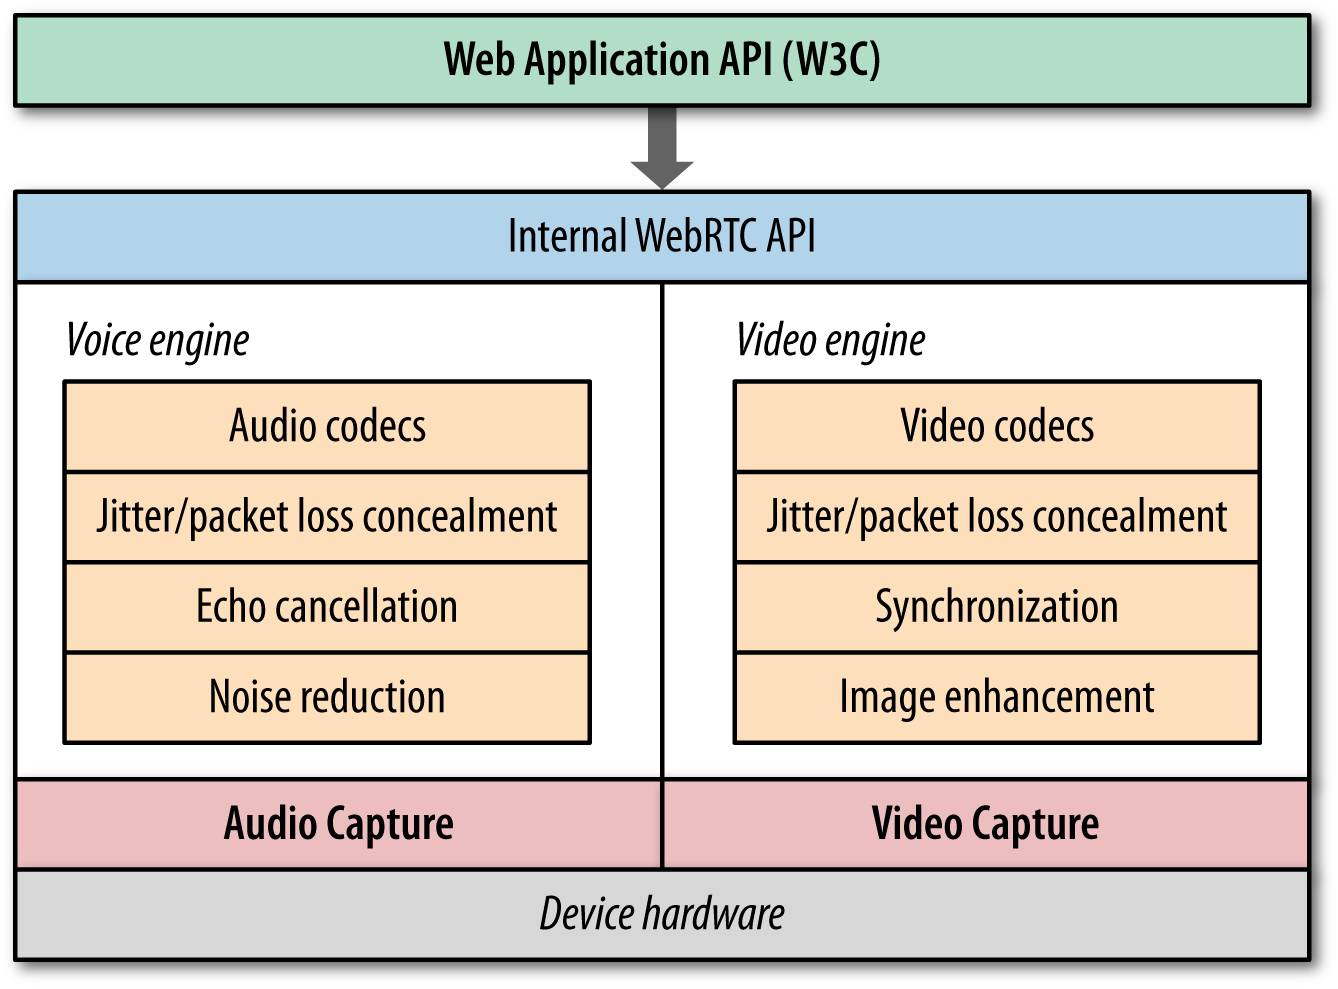
\includegraphics[width=0.9\textwidth]{audio-video_engines}
\caption{Motores de audio y vídeo de WebRTC }
\label{fig:audio-video_engines}
\end{figure}

\emph{getUserMedia} es la API que suministra las funciones y los motores necesarios para poder cumplir con las especificaciones anteriormente mencionadas, así como manipular o procesar los flujos obtenidos. El objeto \textit{MediaStream} (figura \ref{fig:mediaStream}) es la forma en la que nos suministra los flujos esta API.\\

\begin{itemize}
\item El objeto MediaStream consiste en una o varias pistas o \textit{tracks} (\textit{MediaStreamTrack}).
\item Las pistas que componen el MediaStream están sincronizadas una con la otra.
\item La salida del MediaStream puede ser enviada a uno o varios destinatarios, como fuente de vídeo local, un par remoto o procesarlo con funcionalidades que nos proporciona, por ejemplo, HTML5.
\end{itemize}

\begin{figure}[h!]
\centering
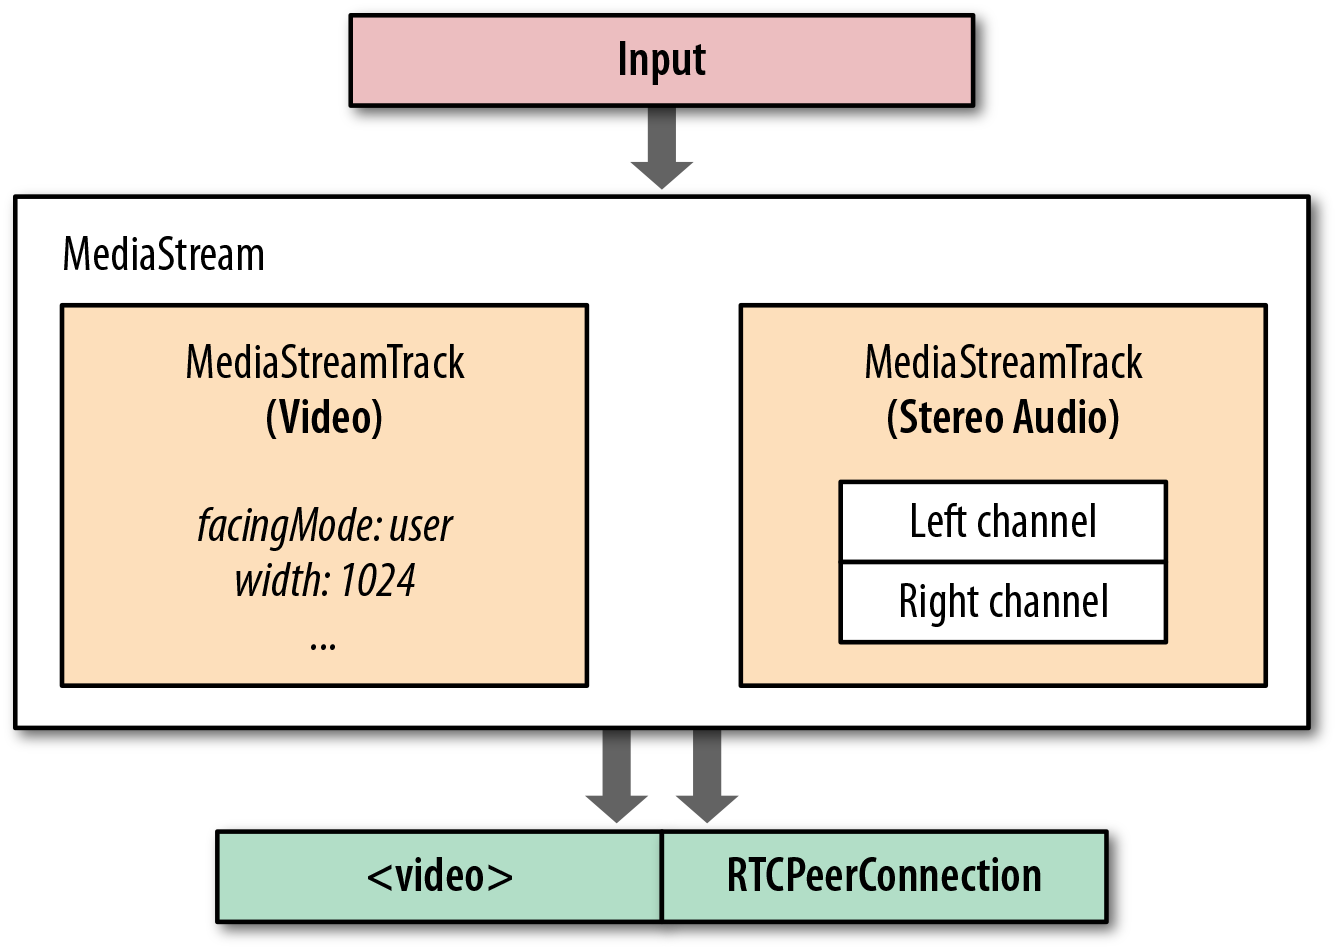
\includegraphics[width=0.9\textwidth]{mediaStream}
\caption{MediaStream}
\label{fig:mediaStream}
\end{figure}

Todo el procesado de audio y vídeo, como la cancelación de ruido, ecualización, mejora de la imagen y todas las demás son automáticamente manejadas por los motores de audio y vídeo.\\

Sin embargo, las características del flujo audiovisual son restringidas por las capacidades de los dispositivos de entrada: audio mono o stereo, diferentes resoluciones de vídeo según la cámara, etc. Cuando hacemos una petición de media al navegador, \emph{getUserMedia} nos permite indicar una lista de restricciones obligadas y opcionales.\\

\begin{lstlisting}[caption=Llamada a función RTCPeerConnection]
var constraints = {
    audio: false,
    video: {
        width: { min: 1024, ideal: 1280, max: 1920 },
        height: { min: 576, ideal: 720, max: 1080 },
    }
};

navigator.getUserMedia(constraints, handleUserMedia, handleUserMediaError); 

function handleUserMedia(stream){
    var video = document.querySelector('video');
    video.src = window.URL.createObjectURL(stream);
}

function handleUserMediaError(error){
	console.log('getUserMedia error: ', error);
}

\end{lstlisting}

\section{WebRTC: API RTCPeerConnection}

Esta API es la encargada de crear la conexión \emph{Peer-2-Peer} entre el navegador local y el remoto. Trabaja de manera diferente si es el que hace la llamada (\textit{caller}) y el que la recibe (\textit{called}) debido a la señalización oferta/respuesta que ya hemos visto. Para ello hace uso de sus funciones para completar el proceso de señalización descrito anteriormente.\\

\noindent Es también la encargada de manejar la conexión una vez establecida. Entre las funciones automáticas que realiza se encuentran:\\

\begin{enumerate}
\item Ocultamiento de paquetes perdidos.
\item Cancelación de eco.
\item Adaptación del ancho de banda.
\item \emph{Buffer} dinámico en función del tembleque (\emph{jitter}) o retardo( \emph{delay}).
\item Control automático de ganancia.
\item Reducción o eliminación de ruido.
\end{enumerate}

Es el desarrollador de la aplicación el encargado de llamar a las funciones que componen esta API en el orden, tiempo y forma correcta para cumplir con la arquitectura JSEP y conseguir un intercambio de descriptores de sesión y de Candidatos ICE exitoso.\\

\noindent La función admite dos argumentos opcionales: \\

\begin{lstlisting}[caption=Llamada a función RTCPeerConnection]
var PC = new RTCPeerConnection(ICEconfig, pcConstraints);
\end{lstlisting}

\textit{ICEConfig} es una variable la cuál contiene los datos necesarios para conectarse con el servidor STUN y TURN y poder hacer NAT Trasversal. \textit{pcConstraints} también es una variable a la que se le pueden añadir una serie de restricciones como \textit{RtpDataChannels}, la cuál estará obsoleta en futuras versiones y se dejará de usar. Esta variable está para futuras mejoras.\\

\begin{normalsize}
\noindent \textbf{Protocolos de transporte en tiempo real}\\
\end{normalsize}

El cerebro humano es muy bueno 'rellenando huecos' pero altamente sensible a los retardos. Si perdemos unas muestras de audio o vídeo no nos afecta demasiado en la percepción de lo que estamos recibiendo, pero en cambio añade un retardo al audio con respecto al vídeo y hará que ese material nos sea hasta molesto.\\

Por este motivo las aplicaciones de audio y vídeo en tiempo real están diseñadas para tolerar pérdidas intermitentes de paquetes. Los codecs pueden rellenar estos pequeños espacios que dejan los paquetes perdidos, muchas veces incluso con muy poco impacto con respecto a la imagen real. Una baja latencia y vicacidad son mucho mas importantes que la fiabilidad (\emph{reliability}).\\

Este requerimiento de vivacidad antes que fiabilidad es la primera razón por la que el protocolo UDP es elegido para el envío de datos en tiempo real. TCP es fiable y tiene entrega ordenada de paquetes. Si uno de ellos se pierde, entonces TCP almacena los paquetes siguientes y para la retransmisión hasta que el paquete perdido es reenviado y recibido. En cambio UDP no garantiza la entrega de paquetes, el orden de entrega, la ruta de los paquetes ni control de congestión de red.\\

WebRTC usa UDP como protocolo de transporte. Dadas las características de UDP, ¿podemos simplemente enviar cada paquete según llega y olvidarnos? no, ya que también necesitamos mecanismos para atravesar NAT's y cortafuegos, negociar los parámetros de cada flujo, encriptar los datos de usuario, congestión de red... Para abastecer estas necesidades WebRTC tiene una lista de protocolos y servicios que trabajan por encima de UDP [(figura \ref{fig:pila_webrtc})].\\

\begin{figure}[h!]
\centering
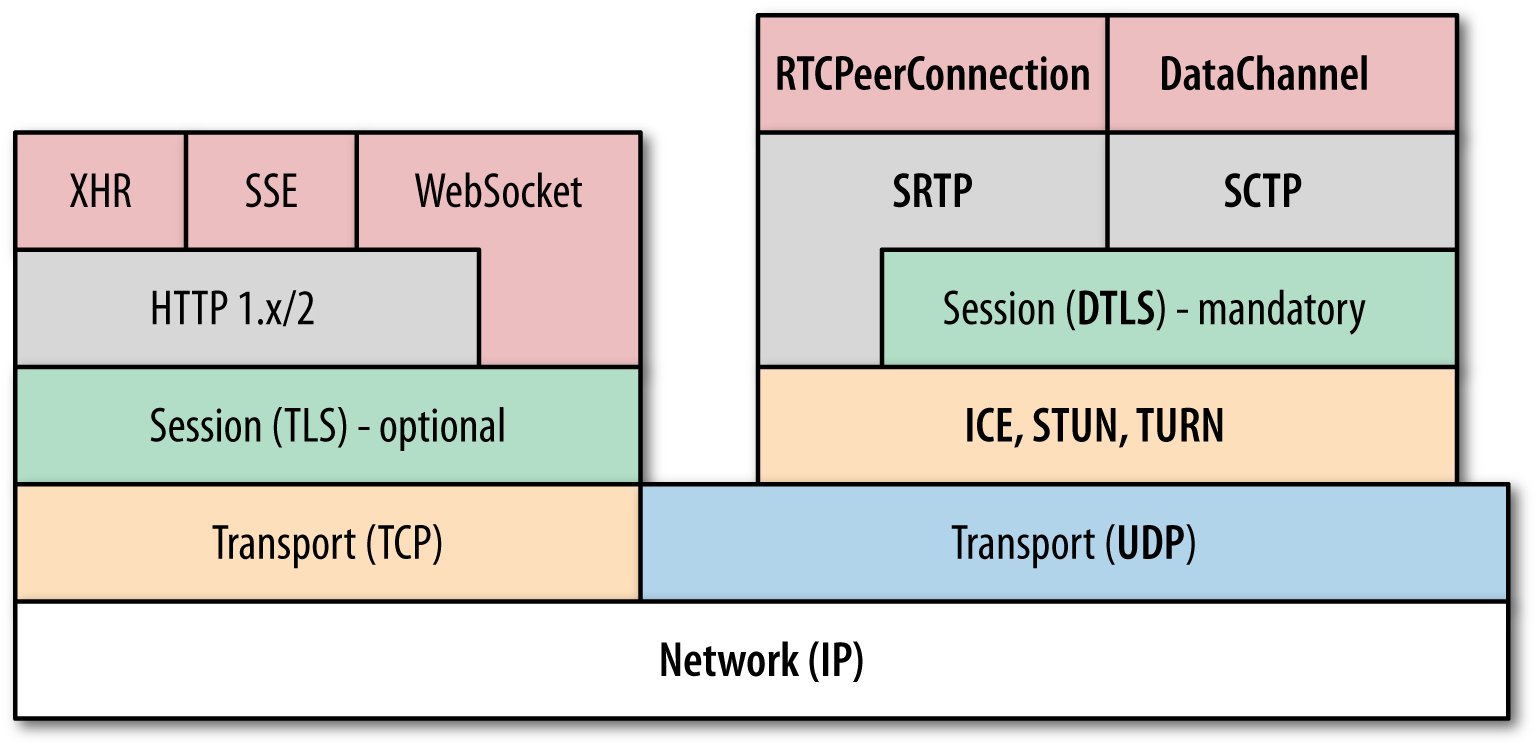
\includegraphics[width=0.9\textwidth]{pila_webrtc}
\caption{Pila de protocolos WebRTC}
\label{fig:pila_webrtc}
\end{figure}


ICE, STUN y TURN son necesarios para establecer y mantener la conexión \emph{Peer-2-Peer} sobre UDP, como ya hemos visto en el apartado de señalización.\\

\begin{normalsize}
\noindent \textbf{Entrega de vídeo con SRTP}\\
\end{normalsize}

WebRTC nos permite adquirir el vídeo/audio y enviarlo para la visualización en el otro par. También nos permite elegir las características con las que queremos adquirir ese vídeo/audio, pero a partir de ahí es WebRTC y el motor de red el que se encarga del resto. Optimización en la codificación, tratar con paquetes perdidos, tembleque, etc, son algunas de las cosas con las que tiene que tratar WebRTC. Por este motivo WebRTC no garantiza la entrega en el otro par del vídeo a su máxima resolución.\\

El motor de red tiene su propio flujo de datos sin tener en cuenta desde el comienzo la capacidad de la red ni el caudal del flujo. Primero empieza enviando el vídeo y el audio a un bitrate bajo (por debajo de 500kbps) y luego comienza a ajustar la calidad del flujo según la capacidad del ancho de banda. Según pueda variar el ancho de banda de la conexión de red así actúa el motor de red para ajustarlo.\\

SRTP (\emph{Secure Real-time Transport Protocol}) es el protocolo que nos proporciona multiplexación de los diferentes flujos y nos proporciona control del flujo y de congestión. Define un formato de paquete estándar para enviar audio y vídeo a través de IP, pero por si mismo no proporciona ningún mecanismo o garantías de entrega en orden, fiabilidad en la entrega o corrección de errores. Simplemente encapsula el vídeo y el audio con metadata adicional. Entre esta metadata cada paquete SRTP tiene un número de secuencia incremental, una marca de tiempo y un identificador SSRC, lo que permite al par que recibe el flujo detectar si los paquetes llegan desordenados, sincronizar los diferentes flujos y asociar cada paquete al flujo correspondiente.\\

SRTP usa un protocolo que lo complementa. Este es SRTCP, el cual es el protocolo que controla el número de paquetes y bytes perdidos, último número de secuencia recibido, \emph{jitter} de los paquetes SRTP recibidos y otras estadísticas. Periódicamente estas estadísticas se intercambian entre los pares y la usan para ajustar la tasa de envío, calidad de codificación y otros parámetros.\\

Ambos protocolos corren directamente sobre UDP y trabajan conjuntamente para adaptar y optimizar la conexión.\\


\section{WebRTC: API RTCDataChannel}

Llegamos a la tercera API de WebRTC. RTCDataChannel nos da la posibilidad de transferir todo tipo de datos u objetos a través de la conexión entre pares establecida con RTCPeerConnection.\\

Esta conexión de datos es \textit{full duplex} y nos permite el intercambio de datos, intercambio de archivos, sincronización de juegos online, etc, todo ello con un retardo mínimo. Las posibilidades son infinitas y se puede adaptar a cualquier necesidad que se tenga para nuestra aplicación.\\

\begin{normalsize}
\noindent \textbf{Capacidades}\\
\end{normalsize}

RTCDataChannel soporta un juego muy flexible de tipos de datos. Soporta \textit{strings}, binarios de JavaScript, \textit{Blobs}, \textit{ArrayBuffer} y \textit{ArrayBufferView}. Según nuestras necesidades nos puede resultar más útil un tipo de datos u otro.\\

Como protocolo de transporte soporta TCP, UDP y SCTP. Esto nos permite configurar la conexión de datos de manera fiable (\textit{reliable}) o no fiable (\textit{unreliable}). La primera de ellas nos garantiza la entrega de todos los mensajes que enviemos y que los mismos lleguen en el mismo orden que los hemos enviado. Esto provoca una sobrecarga que puede provocar un funcionamiento más lento además de tener una mayor sobrecarga. La segunda reduce la sobrecarga dando lugar a tener una conexión más fluida y rápida. SCTP es un protocolo de transporte similar a TCP y UDP que puede funcionar directamente en la cima del protocolo IP. Sin embargo, en WebRTC, SCTP es construido sobre un túnel DTLS, el cuál corre encima de UDP.

\begin{figure}[h!]
\centering
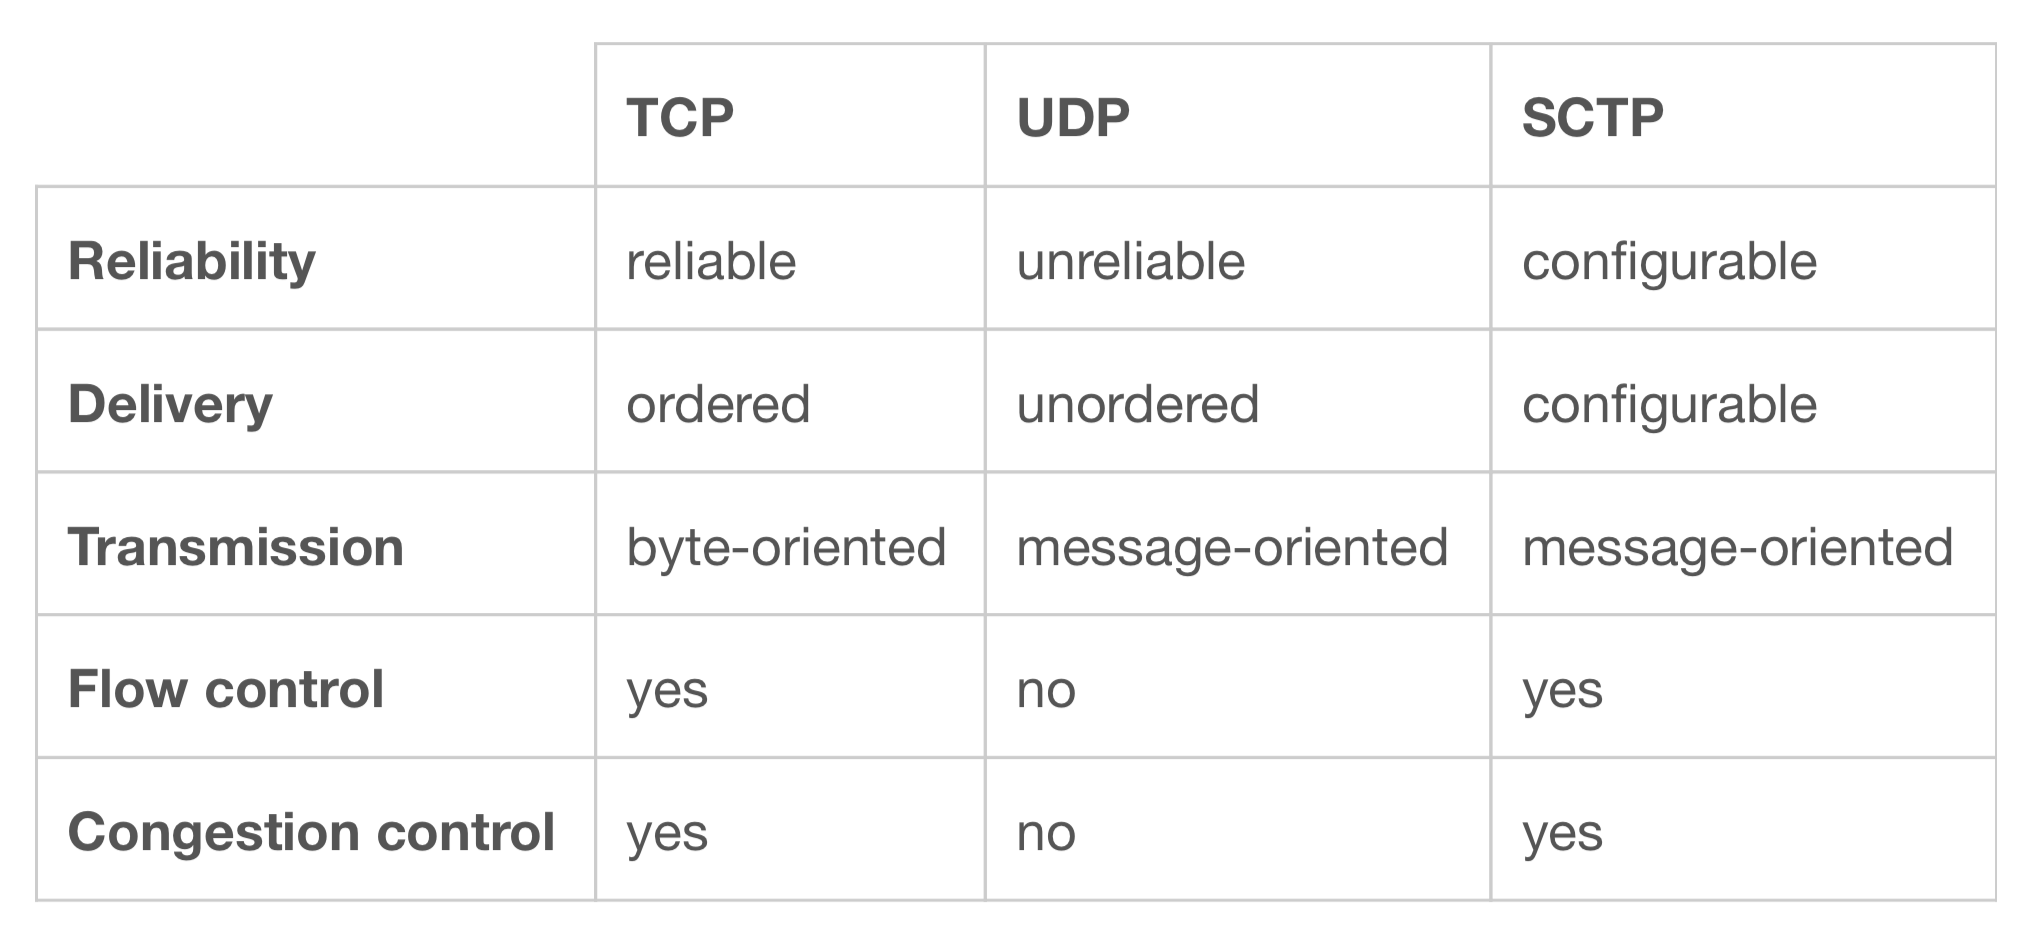
\includegraphics[width=0.9\textwidth]{RTCDataChannel_Capabilities}
\caption{Capacidades de RTCDataChannel.}
\label{fig:datachannel_capabilities}
\end{figure}

\noindent Como las API's anteriores llamamos a RTCDataChannel con una variable para las opciones de configuración:

\begin{itemize}
\item \emph{Ordered}: Booleano para indicar si queremos que nos garantice la entrega ordenada de paquetes.
\item \emph{maxRetransmitTime}: Tiempo máximo para intentar retransmitir cada paquete si la entrega falla. (Fuerza el modo no fiable).
\item \emph{maxRetransmits}: Número máximo de veces que queremos que reenvíe cada paquete si la entrega falla. No puede usarse junto con \textit{maxRetransmitTime}. (Fuerza el modo no fiable).
\item \emph{Protocol}: Permite el uso de un subprotocolo pero tiene que ser soportado por TCP/UDP.
\item \emph{Negociated}: Si se configura a verdadero, elimina la configuración automática del \emph{datachannel} en el otro par. Se da por hecho que tienes previsto crear el canal de otra manera con el mismo ID.
\item \emph{Id}: Permite dar tu propio ID al canal.
\end{itemize}

\begin{normalsize}
\noindent \textbf{Seguridad}\\
\end{normalsize}

La encriptación es una obligación para todos los componentes WebRTC. Tanto audio, vídeo, data e información de la aplicación deben estar encriptados cuando se transmiten. En \emph{RTCDatachannel} todos los datos son codificados con \textit{Datagram Transport Layer Security (DTLS)}. DTLS es un derivado de SSL por lo que los datos que intercambies irán igual de seguro que si usásemos SSL. Es obligatorio, para que un navegador pueda usar WebRTC, que tenga implementada esta tecnología.\\


\begin{normalsize}
\noindent \textbf{Entrega de datos con SCTP}\\
\end{normalsize}

Como ya hemos visto en la figura \ref{fig:pila_webrtc}, \emph{RTCDataChannel} trabaja con un protocolo llamado \textit{Stream Control Transmission Protocol (SCTP)}, el cual corre sobre DTLS, y este a su vez corre sobre UDP. Recalco esto ya que a diferencia del audio y el vídeo, para enviar data de la aplicación sí que necesitamos que lleguen todos los paquetes, por lo que si alguno se ha perdido hay que reenviarlo.\\

\noindent WebRTC requiere de 4 características que debe cumplir el protocolo:

\begin{enumerate}
\item El protocolo de transporte debe permitir tener varios canales independientes multiplexados.
\begin{enumerate}
\item Cada canal debe permitir entrega ordenada y desordenada.
\item Cada canal debe tener entrega fiable.
\item Cada canal debe tener niveles de prioridad definidos por la aplicación.
\end{enumerate}
\item El protocolo debe proveer 'orientación al mensaje', por lo que debe tener fragmentación y reagrupacion de los datos.
\item El protocolo debe tener mecanismos control del flujo y de la congestión.
\item El protocolo debe tener seguridad y confidencialidad en los datos que se envían.
\end{enumerate}

La última característica se cumple ya que SCTP corre sobre el túnel DTLS, por lo que los datos que enviemos van encriptados y seguros hasta nuestro destinatario. Por otro lado SCTP, como vemos en la tabla \ref{fig:datachannel_capabilities} permite configurar la fiabilidad y la entrega ordenada de paquetes. SCTP también trocea los datos que queremos enviar y los encapsula en paquetes SCTP de 224 bits.\\

Para el control de flujo y de congestión SCTP tiene un saludo inicial similar al de TCP. Ambos usan la misma ventana inicial de congestión así como la misma lógica de crecimiento y decrecimiento para reducir la congestión una vez la comunicación está activa.\\


